\documentclass[UTF8,a4paper]{paper}
\usepackage{ctex}
\usepackage[utf8]{inputenc}
\usepackage{amsmath}
\usepackage{amssymb}
\usepackage{pdfpages}
\usepackage{graphicx}
\usepackage{xcolor}
\title{模式识别作业7}
\author{张蔚桐\ 2015011493\ 自55}
\begin {document}
\maketitle
\section{}
\subsection{}
首先我们定义如下表达式来简化表述
\begin{equation}
\epsilon(i,j)\triangleq\epsilon_i(x_j)\triangleq h_i(x_j)-y(x_j)
\label{1}
\end{equation}
为表述所有分类器对所有样本预测的偏差。

于是对于$m$个单独的分类器,他们的平均均方误差可以定义为
\begin{equation}
E_h=\frac{1}{m}\sum_{i=i}^m[\frac{1}{n}\sum_{j=1}^n(\epsilon(i,j)^2)]
\label{2}
\end{equation}
\begin{equation}
E_{h_B}=\frac{1}{n}\sum_{j=1}^n[\frac{1}{m}\sum_{i=1}^{m}\epsilon(i,j)]^2
\label{3}
\end{equation}
交换求和次序,\ref{2}式可以化为
\begin{equation}
E_h=\frac{1}{n}\sum_{j=i}^n[\frac{1}{m}\sum_{i=1}^m(\epsilon(i,j)^2)]
\label{3}
\end{equation}
因此只需要证明,对于$\forall j $下面式子成立则对应小题可以得到证明
\begin{enumerate}
\item $\displaystyle{\frac{1}{m}(\sum_{i=1}^m\epsilon(i,j))^2 =  \sum_{i=1}^m\epsilon(i,j)^2}$
\item $\displaystyle{\frac{1}{m}(\sum_{i=1}^m\epsilon(i,j))^2 \le  \sum_{i=1}^m\epsilon(i,j)^2}$
\end{enumerate}
显然根据柯西——施瓦茨不等式
\begin{equation}
\frac{1}{m}\sum_{i=1}^m\epsilon(i,j)) \le \sqrt{\frac{1}{m}  \sum_{i=1}^m\epsilon(i,j)^2}
\end{equation}
得到上面(2)式成立,当随机变量相互独立时可以得到
\begin{equation}
E_{h_B}=\frac{1}{n}\sum_{j=1}^n[\frac{1}{m}\sum_{i=1}^{m}\epsilon(i,j)]^2=\frac{1}{n}\sum_{j=1}^n\frac{1}{m}\sum_{i=1}^{m}\epsilon(i,j)^2=E_h
\end{equation}
得到证明
\section{}
\subsection{}
训练的错误率在30次,100次,300次迭代的条件下分别是

训练错误率和测试错误率如图\ref{fig1}所示
\begin{figure}
\centering
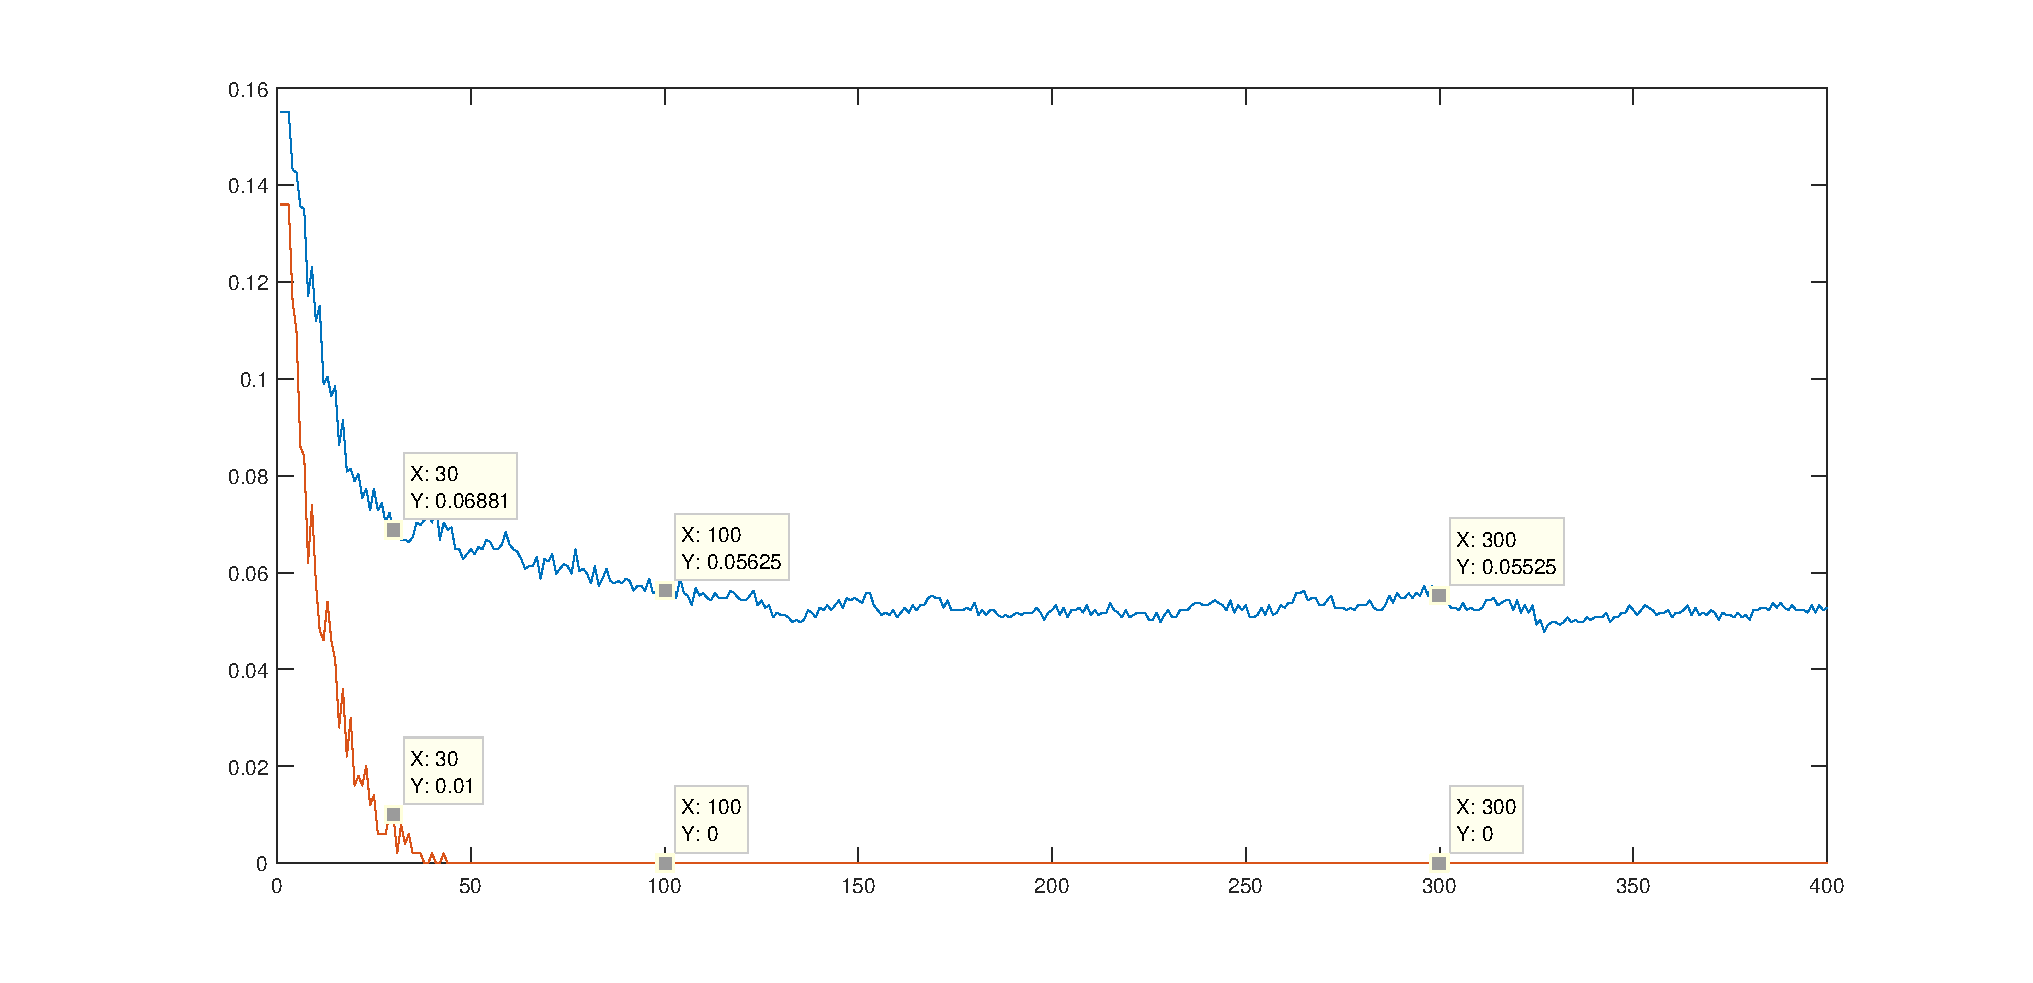
\includegraphics[width=\textwidth]{500trained.eps}
\caption{500个样本的训练错误率和测试错误率}
\label{fig1}
\end{figure}
\end{document}